\section{Estrutura}

Entende-se como o subsistema de estrutura as partes do sistema que possuem função estrutural. Este subsistema é responsável por comportar os demais subsistemas, seguindo os requisitos definidos pelo projeto.

\begin{figure}[H]
\centering
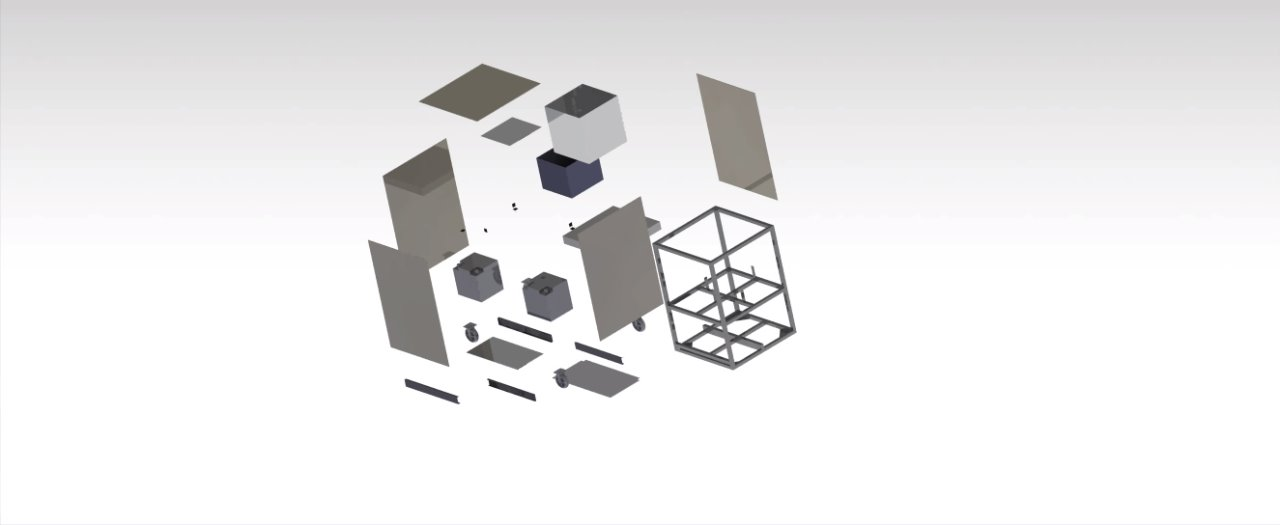
\includegraphics[width=16cm]{figuras/visaoexplodida_estrutura.jpeg}
\caption{Visão explodida}
\end{figure}

\begin{figure}[H]
\centering
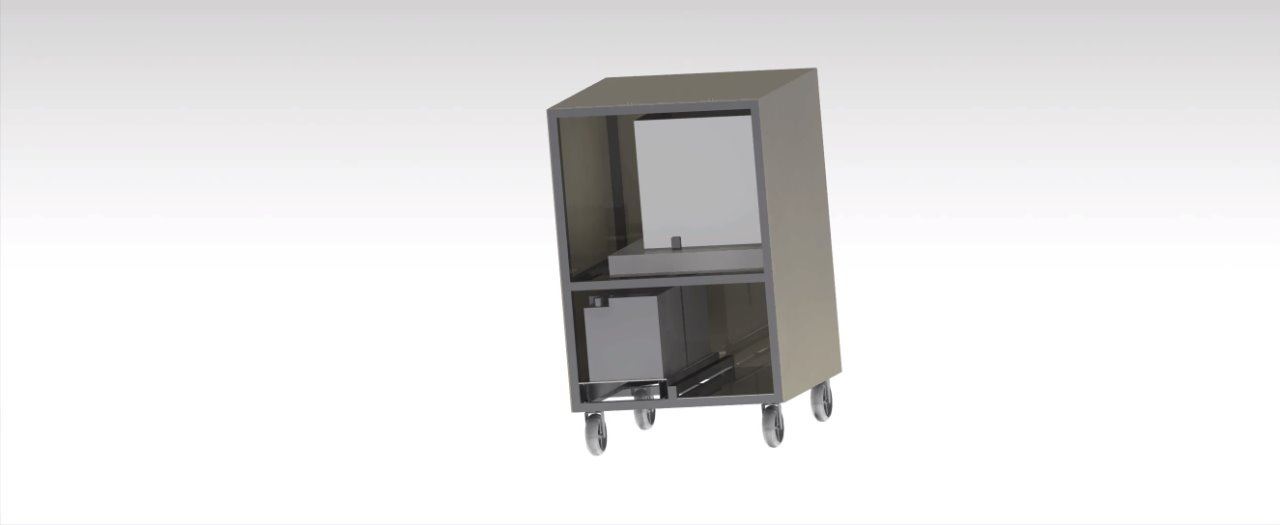
\includegraphics[width=16cm]{figuras/visaolateral_estrutura.jpeg}
\caption{Visão externa lateral}
\end{figure}

\begin{figure}[H]
\centering
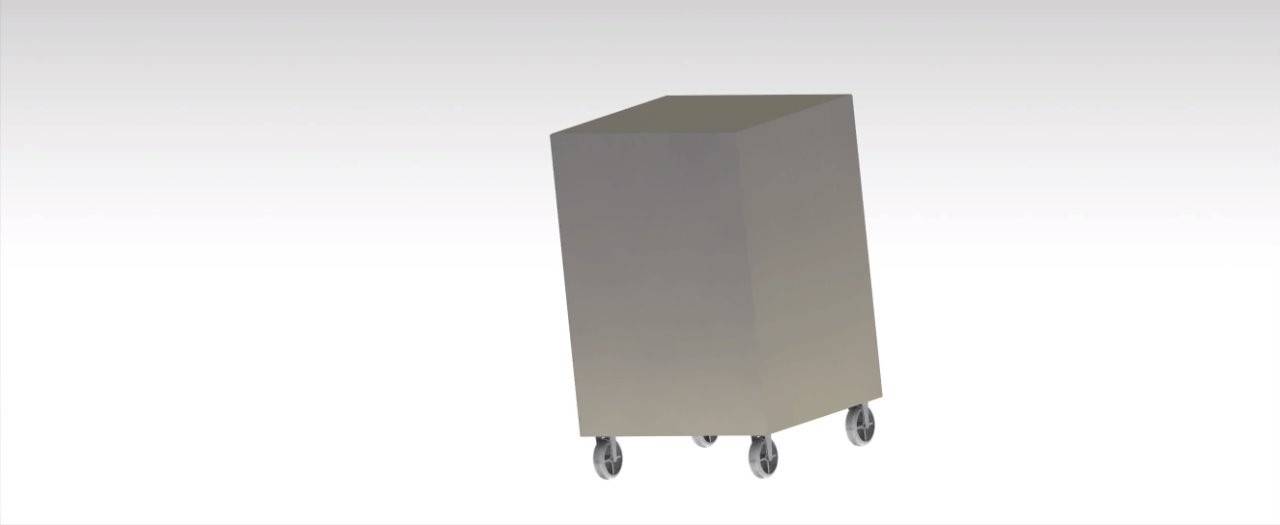
\includegraphics[width=16cm]{figuras/visaoexterna_estrutura.jpeg}
\caption{Visão externa posterior}
\end{figure}

\begin{figure}[H]
\centering
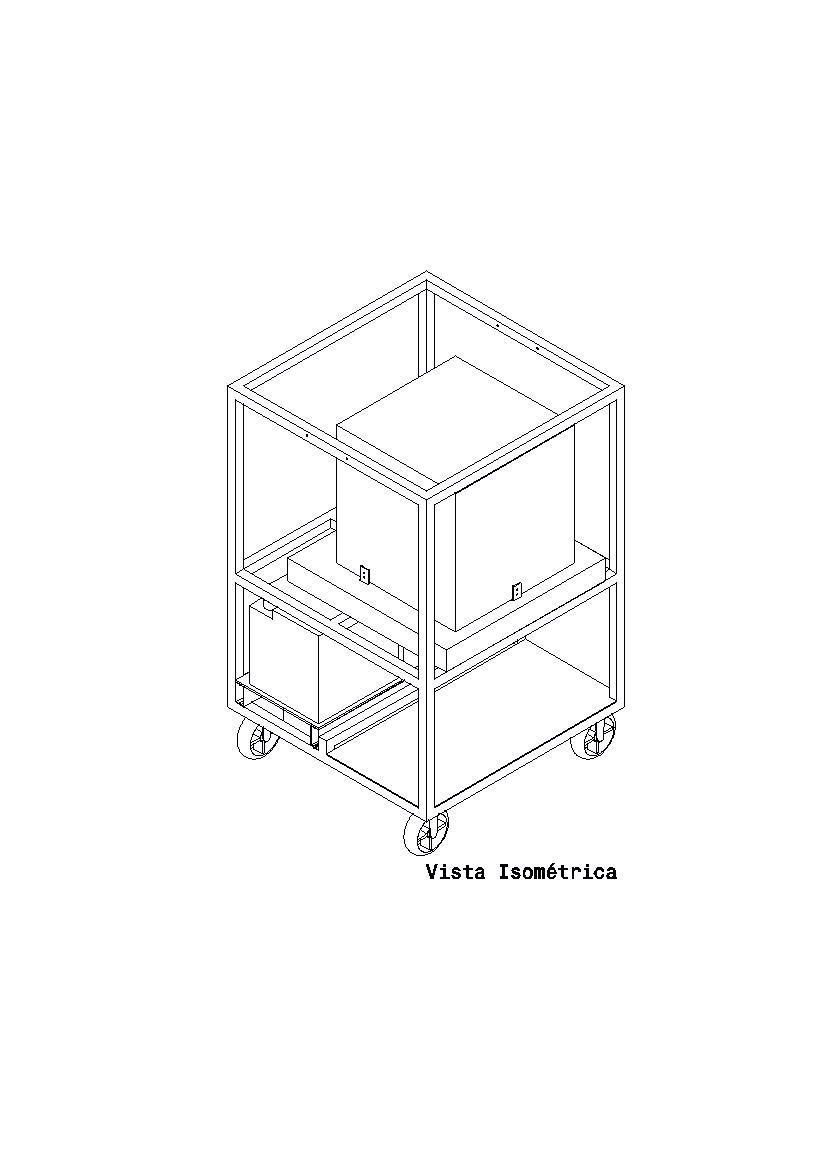
\includegraphics[width=16cm]{figuras/desenhomontagem.png}
\caption{Desenho técnico da estrutura completa}
\end{figure}

\subsection{Componentes Estruturais}

Para fins de melhor compreensão, os componentes da estrutura foram separados em partes, de acordo com suas características e funções.

\subsubsection{Compartimento de carga}

O compartimento de carga, é a caixa mais interna da estrutura, na qual o órgão, dentro das embalagens apropriadas, é transportado.

\paragraph*{Requisitos}\
O compartimento de carga deve ser:

\begin{itemize}
\item Hermeticamente fechado, ou seja, vedado.
\item Facilmente removido ou posicionado na câmara de resfriamento.
\end{itemize}

\paragraph*{Design}\
\begin{itemize}
\item \textbf{Caixa:} De acordo com o tamanho do órgão que será carregado e as embalagens e líquido que estão envolvendo o órgão, e com os requisitos de portabilidade do sistema, o compartimento foi projetado com um design cúbico, para melhor fabricação, dimensionado para ter 24,7 x 24,7 x 20 cm.
\item \textbf{Tampa:} O formato escolhido para a tampa da caixa foi um prato quadrado de 24,7 x 24,7 cm. Deste modo, o compartimento pode ser vedado com a aplicação de tiras de borracha nas bordas da caixa e da tampa. Uma alça posicionada no centro e topo da tampa serve para manusear o compartimento.
\item \textbf{Fixadores:} Para que o compartimento seja hermético, a tampa deve ser bem fixada na caixa. Por isso, foram adicionados 6 presilhas distribuídas ao redor da caixa para prender a tampa.
\end{itemize}

O material escolhido para o compartimento foi aluminio, devido a sua propriedade de alta condutividade térmica, de modo a facilitar o resfriamento do interior do compartimento.

\begin{figure}[H]
\centering
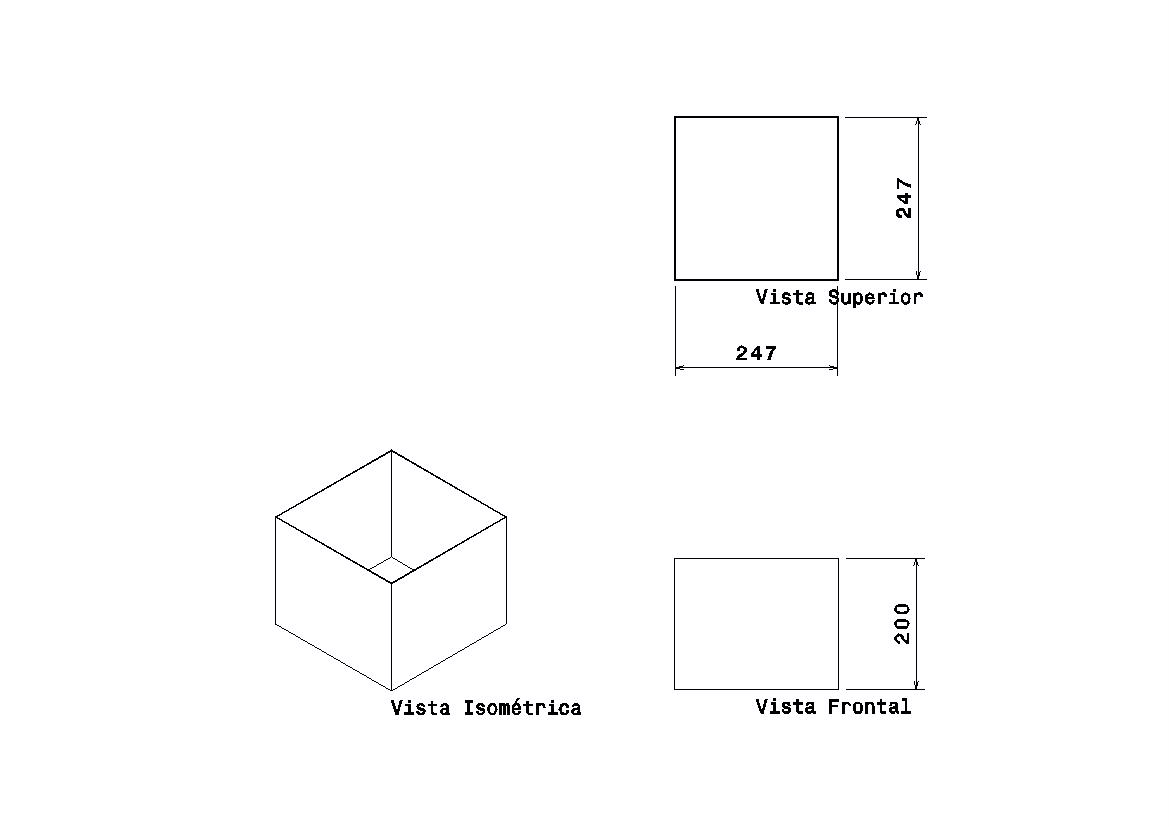
\includegraphics[width=16cm]{figuras/desenhocompartimento.png}
\caption{Desenho técnico do compartimento de carga}
\end{figure}


\paragraph*{Fabricação}\
Os materiais utilizados foram:

\begin{itemize}
\item Chapa de alumínio série 5000 1m X 1m de 2mm espessura
\item Borrachas
\item Presilhas
\item Alça
\end{itemize}

Procedimentos:
\begin{enumerate}
\item Inicialmente, a chapa de alumínio foi cortada utilizando cortadora de chapas.
\item Em seguida, a chapa foi dobrada com 90 graus utilizando a dobradora de chapas.
\item para finalizar a caixa foi soldada utilizando o processo TIG (tungstênio inert gás). 
\item Foi aplicado pasta de silicone nas bordas da caixa e da tampa para ajudar na vedação. Foi fixada então a borracha utilizando cola instantânea.
\item As presilhas foram
\item Enfim, a alça foi posicionada no centro da tampa e rebitada para sua fixação.
\end{enumerate}

\subsubsection{Câmara de Resfriamento}

A câmara de resfriamento é a parte da estrutura resfriada pelo sistema de refrigeração e onde se encontra o compartimento de carga.

\paragraph*{Requisitos}\
A estrutura da câmara de resfriamento deve ser:

\begin{itemize}
\item Isolada termicamente.
\item Capaz de comportar o compartimento de carga e parte interna do sistema de refrigeração.
\item Capaz de apoiar o compartimento de carga de modo fixo, para que este não se movimente com o deslocamento da transportadora.
\item Fixa na estrutura principal, porém seu topo deve ser acessível do lado externo.
\end{itemize}

\paragraph*{Design}\
\begin{itemize}
\item \textbf{Caixa:} Similarmente ao compartimento de carga, a câmara de resfriamento foi projetada com formato cúbico, porém o fundo da caixa é arredondado ao invés de plano para que a água gerada pelo sistema de refrigeração escoe para uma saída localizada no centro do fundo. Foram escolhidas as dimensões de 30 x 30 x 30 cm para a caixa. O material escolhido foi aço inox devido às suas excelentes propriedades de resistência e isolamento térmico.
\item \textbf{Tampa:} A tampa da caixa é composta por uma seção quadrada de 30 x 30 cm de aço inox, contornada com borracha e conectada à caixa por dobradiças em um dos lados. Para abrir a câmara, a tampa possui uma alça.
\item \textbf{Isolamento térmico:} Para que a câmara seja isolada termicamente, esta é cercada por uma camada de 5 cm de isopor comum em todas as faces da caixa.
\item \textbf{Apoios do compartimento de carga:} Para gerar melhor estabilidade para o compartimento de carga, a câmara de combustão possui 4 encaixes em ‘L’ no fundo e 2 apoiadores na tampa para manter a o compartimento em uma posição fixa quando a câmara se encontrar fechada.
\item \textbf{ Fixadores:} Assim como o compartimento de carga, a tampa da câmara de resfriamento é fechada por presilhas. Na câmara são utilizadas 4 presilhas, sendo 2 no lado oposto das dobradiças e 1 em cada lado restante.
\end{itemize}


\begin{figure}[H]
\centering
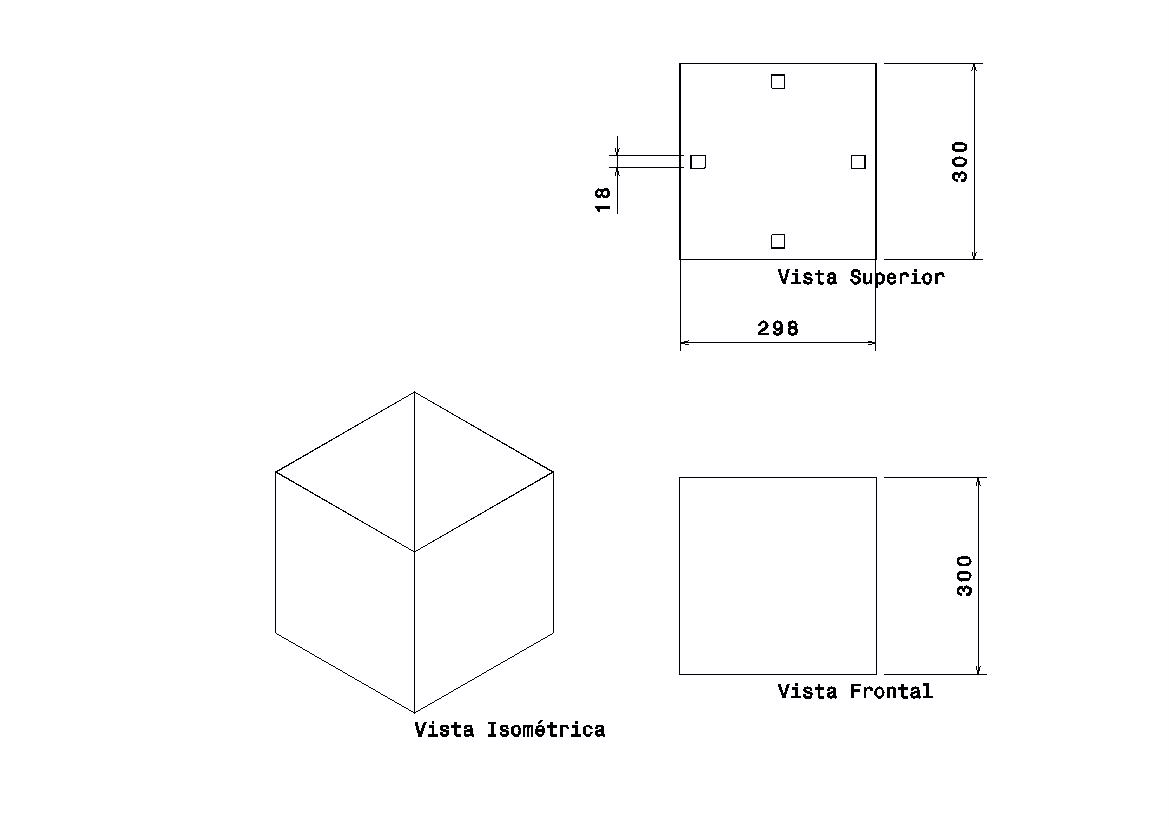
\includegraphics[width=16cm]{figuras/desenhocamara.png}
\caption{Desenho técnico da câmara de resfriamento}
\end{figure}


\paragraph*{Fabricação}\
Materiais Utilizados:

\begin{itemize}
\item Chapa de aço inox 304L 2m X 1m de 1.2mm espessura
\item Placa de Isopor de 5 cm de espessura
\item Borrachas
\item Dobradiças
\item Presilhas
\item Chapa de aço Metalon de 2 mm de espessura
\end{itemize}

Procedimentos:

\begin{enumerate}
\item A chapa de aço foi cortada utilizando cortadora de chapas.
\item Depois, a chapa foi dobrada em ângulos de 90 graus utilizando a dobradora de chapas.
\item A solda foi realizada utilizando o processo TIG (tungstênio inert gás).
\item Em seguida, o fundo da caixa foi amassado para tomar um formato arredondado e foi feito um furo no centro do fundo para escoamento de água.
\item Foram cortadas e soldadas partes de chapa de aço Metalon para formar os apoiadores e estes foram furados e rebitados no fundo da caixa. Foi colado com cola instantânea pedaços de borracha no topo dos apoiadores.
\item As tampas depois de cortadas foram furadas para a colocação das presilhas e as dobradiças de metal. Após a furação foi feita fixação das peças na tampa com rebites.
\item A placa de isopor foi fixada com cola para isopor e silicone industrial transparente na estrutura e na câmara de resfriamento.
\end{enumerate}


\subsubsection{Estrutura}

Define-se aqui como estrutura a parte que de estrutura básica da transportadora, que engloba as demais partes e é responsável pela maior parte da sustentação de forças.

\paragraph*{Requisitos}\
A estrutura deve:
\begin{itemize}
\item Ser capaz de sustentar as forças atuantes sem sofrer deformação considerável.
\item Ter espaço interno capaz de comportar, no mínimo, a câmara de resfriamento, o sistema de refrigeração, duas baterias e os subsistemas eletrônicos.
\end{itemize}

\paragraph*{Design}\
\begin{itemize}
\item \textbf{Estrutura:} Foi projetada uma estrutura composta por barras de aço de seção quadrada de 20 x 20 mm e 1,2mm de espessura. Uma configuração de duas partes foi adotada, na qual a parte superior comporta a câmara de resfriamento e os sistemas eletrônicos, e a interior comporta o compressor e as baterias. 
\item \textbf{Fixadores:} Para fixar a câmara de resfriamento em seu lugar na estrutura, 4 peças em formato “L” foram posicionadas de modo que um lado do fixador será preso na estrutura, e o outro lado na câmara.
\item \textbf{Base:} Para sustentar a parte externa do sistema de refrigeração e a bateria, uma placa de alumínio será fixada no fundo da parte inferior da estrutura.
\item \textbf{Rodas}: Para a movimentação da transportadora, o sistema tem 4 rodas, com travas, fixas embaixo da estrutura por placas triangulares soldadas nas barras inferiores.
\end{itemize}

\begin{figure}[H]
\centering
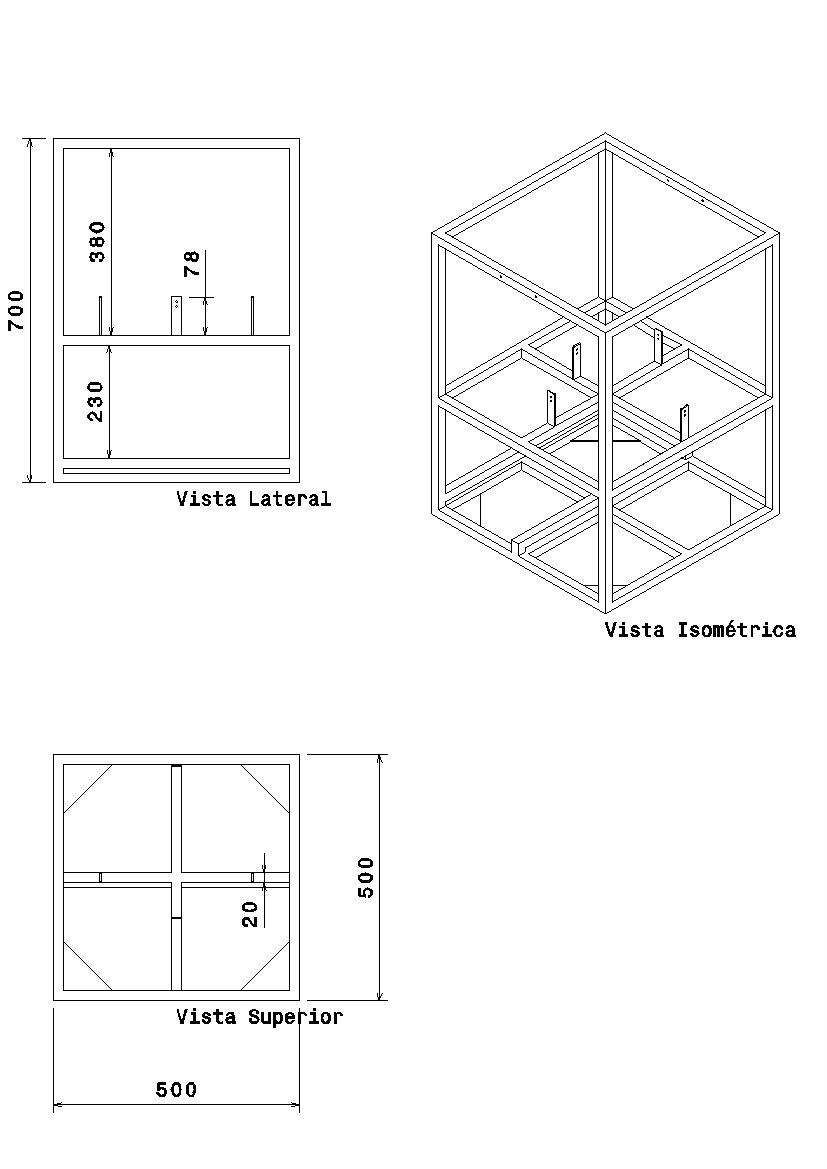
\includegraphics[width=16cm]{figuras/desenhoestrutura.png}
\caption{Desenho técnico da estrutura}
\end{figure}

\paragraph*{Fabricação}\
Materiais Utilizados:
\begin{itemize}
\item Aço estrutural Metalon 20 x 20 x 1,2 mm
\item Chapa de aço carbono de 20x20 1,2 mm de espessura
\item Chapa de aço de 2 mm de espessura
\end{itemize}

Procedimentos:

\begin{enumerate}
\item As barras foram cortadas com a esmerilhadora utilizando um disco próprio para corte do metal. Após cortadas foram corrigidas e acabadas com um esmeril fixo.
\item A solda foi realizada utilizando o processo MIG (metal inert gás) e desbastadas com a máquina esmerilhadora utilizando o disco esmerilhador.
\item Os fixadores da caixa de refrigeração foram soldados na estrutura com um ângulo de 90 graus e esmerilhados para o acabamento da solda.
\item A placa de aço carbono de fixação do sistema compressor foi fixada com rebites nos buracos feitos na estrutura com uma furadeira.
\item As rodas foram fixadas em placas de aço triangulares de 2 mm de espessura soldadas na parte inferior do metalon estrutural. Há borrachas de 3mm de espessura entre a estrutura das rodas e o metalon onde foi fixado com parafusos.
\end{enumerate}


\subsection{Simulação Computacional}

\subsubsection{Análise Estrutural}

O Método dos Elementos dos Elementos Finitos (MEF) é considerado como um método matemático capaz de resolver problemas complexos de forma eficiente e rápida. Lotti (2006), define o MEF como sendo um modelo matemático em meio contínuo que é discretizada em elementos, mantendo as propriedades do objeto em análise. Qualquer falha em componentes estruturais é iniciada após a tensão aplicada exceder o limite de escoamento do material naquele local, Beer e Johnston (1982). Com base nisso utilizaremos o MEF para analisar a viabilidade estrutural do projeto.

Para análise estática cada elemento utilizado na geração da malha é interpretado como uma mola com uma dada rigidez e tamanho determinado. Esta consideração faz com que possamos construir matrizes em termos de carregamento, deslocamentos e rigidez, onde a rigidez depende das propriedades dos materiais e da geometria da peça em análise.

\paragraph*{Condições de Contorno}\
\begin{table}[H]
\centering
\caption{Condições de Contorno da Análise Estrutural}
\label{condcontornoestrut}
\begin{tabular}{|c|c|c|}
\hline
Peça                   & Restrição                                         & Carregamento {[}N{]} \\ \hline
Estrutura              & Engaste na extremidade inferior                   & 120+120              \\ \hline
Compartimento de Carga & Contato fixo nos apoios da câmara de resfriamento & 100                  \\ \hline
Câmara de Resfriamento & Contato fixo nos apoios da estrutura              & --                   \\ \hline
\end{tabular}
\end{table}

\paragraph*{Resultados}\

\begin{figure}[H]
\centering
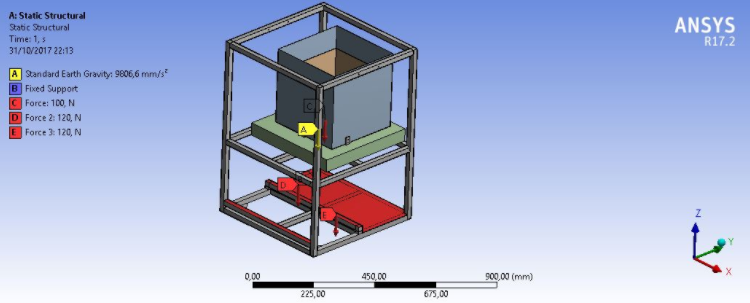
\includegraphics[width=16cm]{figuras/carregamentos.png}
\caption{Carregamentos}
\end{figure}

\begin{figure}[H]
\centering
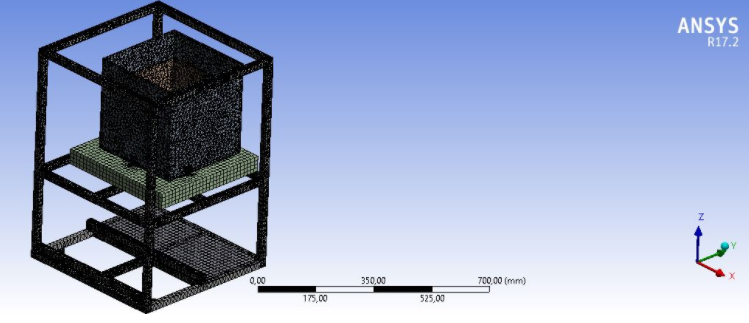
\includegraphics[width=16cm]{figuras/malharefinada.png}
\caption{Refinamento da Malha}
\end{figure}

\begin{figure}[H]
\centering
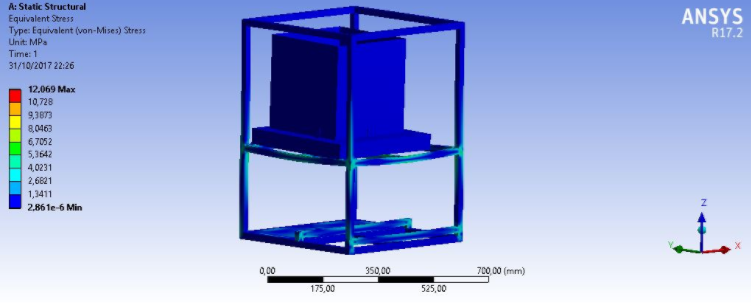
\includegraphics[width=16cm]{figuras/tensaoequivalente.png}
\caption{Tensão Equivalente de Von Mises}
\end{figure}

\begin{table}[H]
\centering
\caption{Resultados para análise estática}
\label{analiseestatica}
\begin{tabular}{|c|c|c|}
\hline
Peça                   & Material & Máxima Tensão Equivalente {[}MPa{]} \\ \hline
Estrutura              & Metalon  & 8,000                               \\ \hline
Compartimento de Carga & Alumínio & 12,069                              \\ \hline
\end{tabular}
\end{table}

\begin{table}[H]
\centering
\caption{Modos de falha e frequências de ressonância}
\label{ressonancia}
\begin{tabular}{|c|c|}
\hline
Modo & Frequência {[}Hz{]} \\ \hline
1    & 40,348              \\ \hline
2    & 41,746              \\ \hline
3    & 63,886              \\ \hline
4    & 79,741              \\ \hline
5    & 86,600              \\ \hline
6    & 100,14              \\ \hline
7    & 101,15              \\ \hline
8    & 117,9               \\ \hline
9    & 118,43              \\ \hline
10   & 122,59              \\ \hline
11   & 143,65              \\ \hline
12   & 150,92              \\ \hline
\end{tabular}
\end{table}

\begin{figure}[H]
\centering
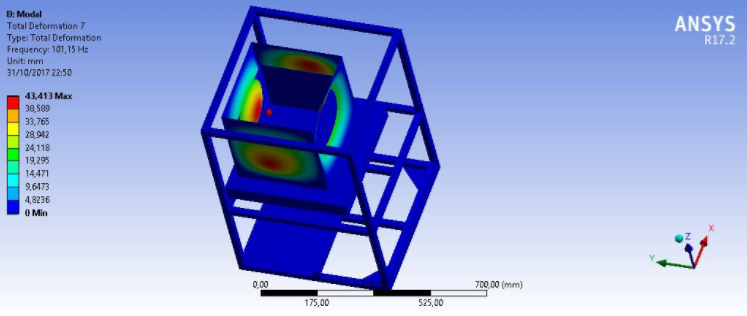
\includegraphics[width=16cm]{figuras/mododefalha7.png}
\caption{Modo de Falha 7}
\end{figure}

\begin{figure}[H]
\centering
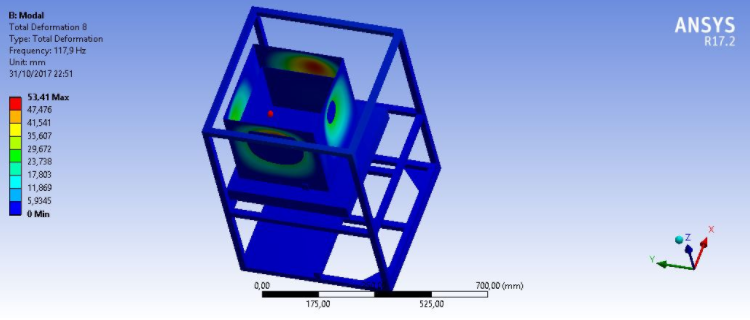
\includegraphics[width=16cm]{figuras/mododefalha8.png}
\caption{Modo de Falha 8}
\end{figure}

\begin{figure}[H]
\centering
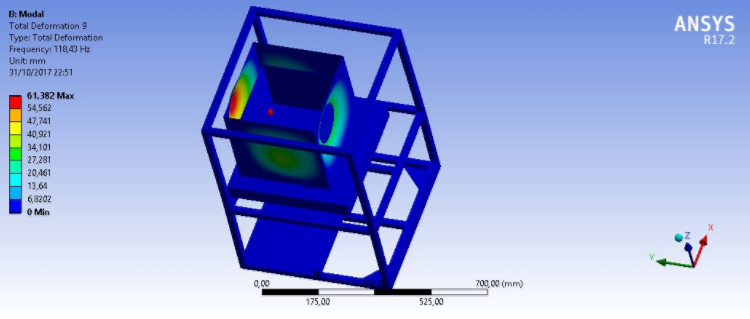
\includegraphics[width=16cm]{figuras/mododefalha9.png}
\caption{Modo de Falha 9}
\end{figure}

\begin{figure}[H]
\centering
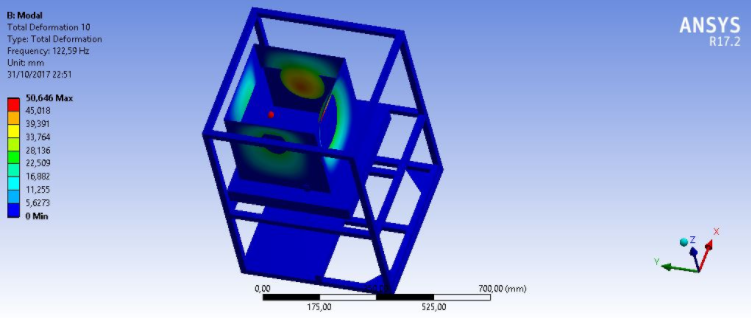
\includegraphics[width=16cm]{figuras/mododefalha10.png}
\caption{Modo de Falha 10}
\end{figure}


\subsubsection{Simulação de Transferência de Calor }

O principal objetivo do projeto é o transporte seguro de órgãos, dentro das condições necessárias. Portanto, um dos pontos mais importantes é a refrigeração do órgão para que este esteja sempre em um ambiente com temperatura dentro dos limites aceitáveis.

É interessante portanto, simular a transferência de calor principalmente no compartimento de carga e na câmara de resfriamento. Para isto, foi desenhado um modelo simplificado desses componentes da estrutura em CAD e foi feita uma simulação em ANSYS Steady Thermal.

O modelo utilizado para a simulação é composto de um cubo representando o compartimento de carga e uma caixa representando a câmara de resfriamento, dentro da qual está a serpentina do sistema de refrigeração.

\paragraph*{Condições de contorno}\

\begin{itemize}
\item Temperatura inicial do compartimento de carga: 2 graus C.
\item Temperatura inicial da câmara de resfriamento: 0 graus C.
\item Temperatura dos ambientes de convecção: 0 graus C.
\item Temperatura na entrada da serpentina: -10 graus C.
\item Temperatura na saída da serpentina: 0 graus C.
\end{itemize}

A transferência de calor é feita da serpentina para a caixa por convecção com coeficiente de convecção $h = 48,83 W/m^2K$ e da câmara de resfriamento para o compartimento de carga com coeficiente $h = 40 W/m^2K$.

\paragraph*{Resultados}\

\begin{figure}[H]
\centering
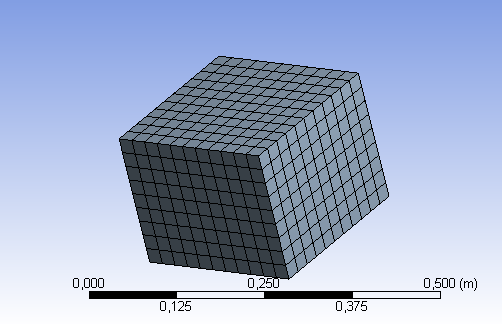
\includegraphics[width=16cm]{figuras/meshcompartimento.PNG}
\caption{Malha do compartimento de carga}
\end{figure}

\begin{figure}[H]
\centering
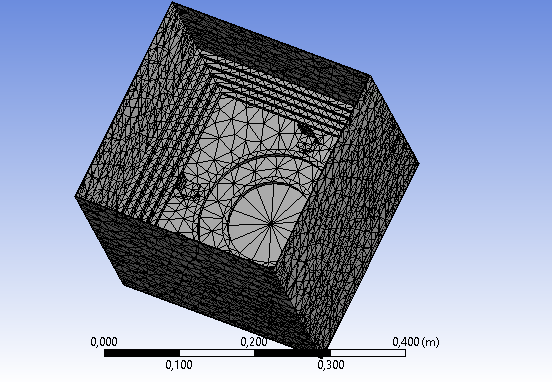
\includegraphics[width=16cm]{figuras/meshcamara.PNG}
\caption{Malha da câmara de resfriamento}
\end{figure}

\begin{figure}[H]
\centering
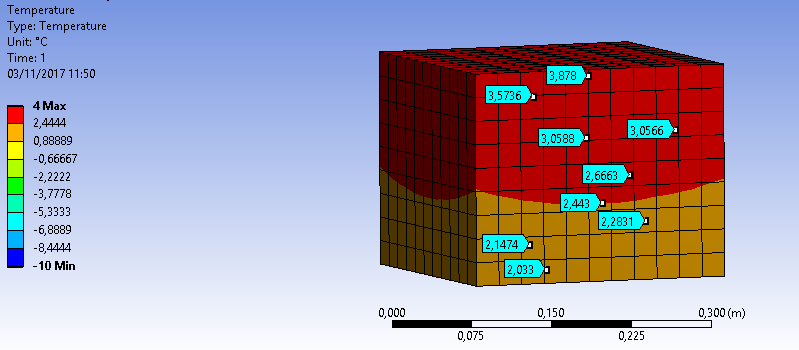
\includegraphics[width=16cm]{figuras/tempcompartimento.PNG}
\caption{Distribuição de temperatura no compartimento de carga}
\end{figure}

\begin{figure}[H]
\centering
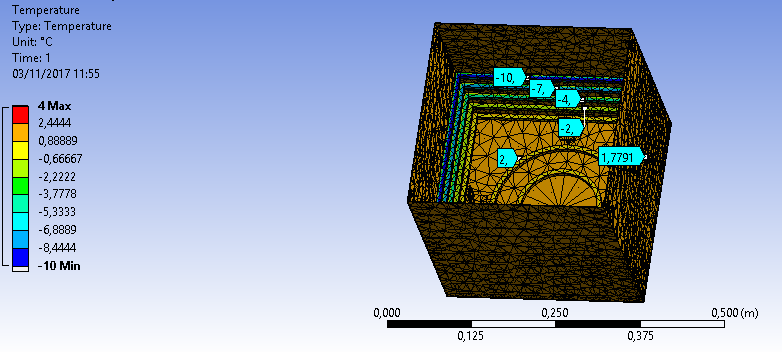
\includegraphics[width=16cm]{figuras/tempcamara.PNG}
\caption{Distribuição de temperatura na câmara de resfriamento}
\end{figure}

\begin{figure}[H]
\centering
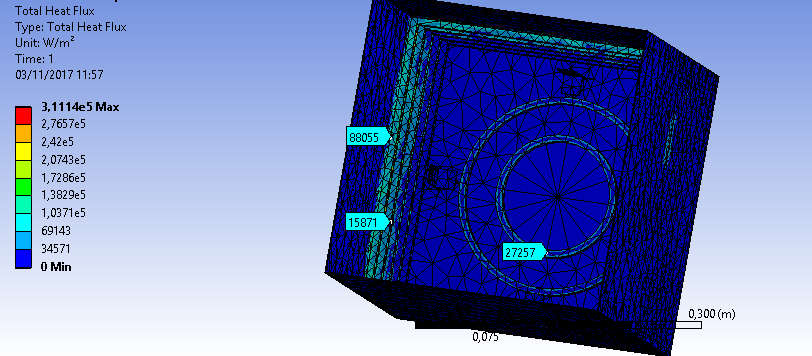
\includegraphics[width=16cm]{figuras/fluxocamara.PNG}
\caption{Fluxo de calor na câmara de resfriamento}
\end{figure}


